%%=============================================================================
%% Onderzoek
%%=============================================================================

\chapter{Vergelijkend Onderzoek}
\label{ch:vergelijkendonderzoek}
In dit deel van het onderzoek zal er van de twee eerder opgebouwde datamodellen een vergelijking gemaakt worden. Hierbij wordt voornamelijk gefocust op deze 5 pijlers:

\begin{itemize}
	\item \textbf{Performantie:} is er een significant verschil in uitvoeringstijd en bij het inladen van gegevens?
	\item \textbf{Complexiteit:} zijn beide modellen makkelijk interpreteerbaar door IT \& business?
	\item \textbf{Flexibiliteit:} hoe flexibel zijn beide modellen wanneer een business requirement gewijzigd wordt?
	\item \textbf{Schaalbaarheid:} hoe gaan beide modellen overweg met enorme hoeveelheid data?
	\item \textbf{Audit:} is er metadata beschikbaar over de werkelijke data? Kunnen problemen makkelijk opgespoord worden?
\end{itemize} 

Op basis van deze resultaten zal er kunnen opgemaakt worden of de keuze voor Data Vault wel de juiste keuze was voor dit project.

\section{Performantie}
Wanneer we de performantie vergelijken tussen twee data warehouses, kan dit gebeuren op twee vlakken: op vlak van het lezen van data, en op vlak van het inladen van de data.

Het inladen van data zal sneller gebeuren bij het Data Vault model. Dit omdat Data Vault toelaat data parallel in te laden. Dit komt omdat de tabellen binnen dit model niet afhankelijk zijn van elkaar. Bij het dimensioneel model is dit een ander verhaal, hierbij moeten de dimensions eerst ingeladen, dan de fact tabel. 

Leesoperaties gebeuren veel performanter op het dimensioneel model. Dit komt omdat het dimensioneel model veel minder relaties bevat en dus veel minder joins zal moeten maken om alle benodigde data te verkrijgen. Wanneer een join gebeurt, zorgt dit toch wel voor vertraging. Het Data Vault model bestaat uit veel meer tabellen, dus zullen er heel wat meer joins moeten gebeuren om de benodigde data te lezen. 

Qua performantie kunnen er dus 2 zaken geconcludeerd worden: Data Vault is heel performant in het inladen van gegevens, maar het inlezen van data gebeurt veel performanter bij het dimensioneel model.

\section{Complexiteit}
Bij het modelleren van data kan complexiteit ontstaan zowel bij het interpreteren van het data model als bij het opmaken van het data model. 

Wanneer de business of de IT een dimensioneel model moet interpreteren, zal dit gemakkelijker gaan in vergelijking met een Data Vault model. Bij een dimensioneel model zijn veel minder relaties, dat zorgt voor een overzichtelijker schema. Ook komt alles samen in één centraal punt (fact), waaraan alles gelinkt is. Bij het interpreteren van een Data Vault model, moet die persoon al beschikken over kennis over Data Vault. Hij/zij moet weten wat het doel is van de verschillende soorten tabellen (hubs, links \& sattelites). Ook zullen de vele verschillende entiteiten samen het overzicht belemmeren. 

De transactionele gegevens staan bij het dimensioneel model altijd gecentraliseerd op één plaats. Zo is het zeer eenvoudig om te weten te komen welke transactionele gegevens (en business logica) er gebruikt wordt. Dit is niet altijd het geval bij Data Vault. In dit onderzoek staan die gegevens toevallig wel samen op één plaats, maar in de praktijk zal dit niet altijd het geval zijn. Dan worden de transactionele gegevens bij een Data Vault model samengevoegd in een data mart.

Als een datamodel ontworpen wordt aan de hand van het dimensioneel modelleren, kan er snel en gemakkelijk tot een resultaat bekomen worden in vergelijking met Data Vault. Bij het ontwerpen van een dimensioneel model wordt er gestart vanuit de dimensions, die leiden naar één centraal punt, de fact. Wanneer een Data Vault model dient ontworpen te worden, kan dit op veel verschillende manieren gebeuren. Er wordt gestart vanuit hubs, die de pilaren vormen voor het model, daarna worden deze verbonden met elkaar aan de hand van links. Finaal wordt beslist welke sattelites zullen aangemaakt worden en aan welke hubs/links deze gekoppeld zullen worden.

Wanneer historisatie een requirement is, dan heeft Data Vault een streepje voor op het dimensioneel modelleren. Bij Data Vault zit historisatie al in het model geïntegreerd, bij het dimensioneel modelleren niet. Er kan geopteerd worden voor historisatie bij het dimensioneel modelleren door gebruik te maken van slow changing dimensions, maar dit verhoogt wel aanzienlijk de complexiteit van het model.

Op vlak van complexiteit, kan er geconcludeerd worden dat Data Vault een hogere complexiteit bevat dan in vergelijking met het dimensioneel model, zowel op het vlak van het model interpreteren als het opstellen van een nieuw model.

\section{Flexibiliteit}
Bij het toevoegen van nieuwe requirements, moet er bij Data Vault nieuwe hub(s) ontworpen en geïmplementeerd worden samen met de daarbij horende links/sattelites. Indien daarbij nieuwe businesslogica wordt bijgevoegd, kan deze in de nieuwe sattelites geplaatst worden. 

\begin{figure}[h]
	\centering
	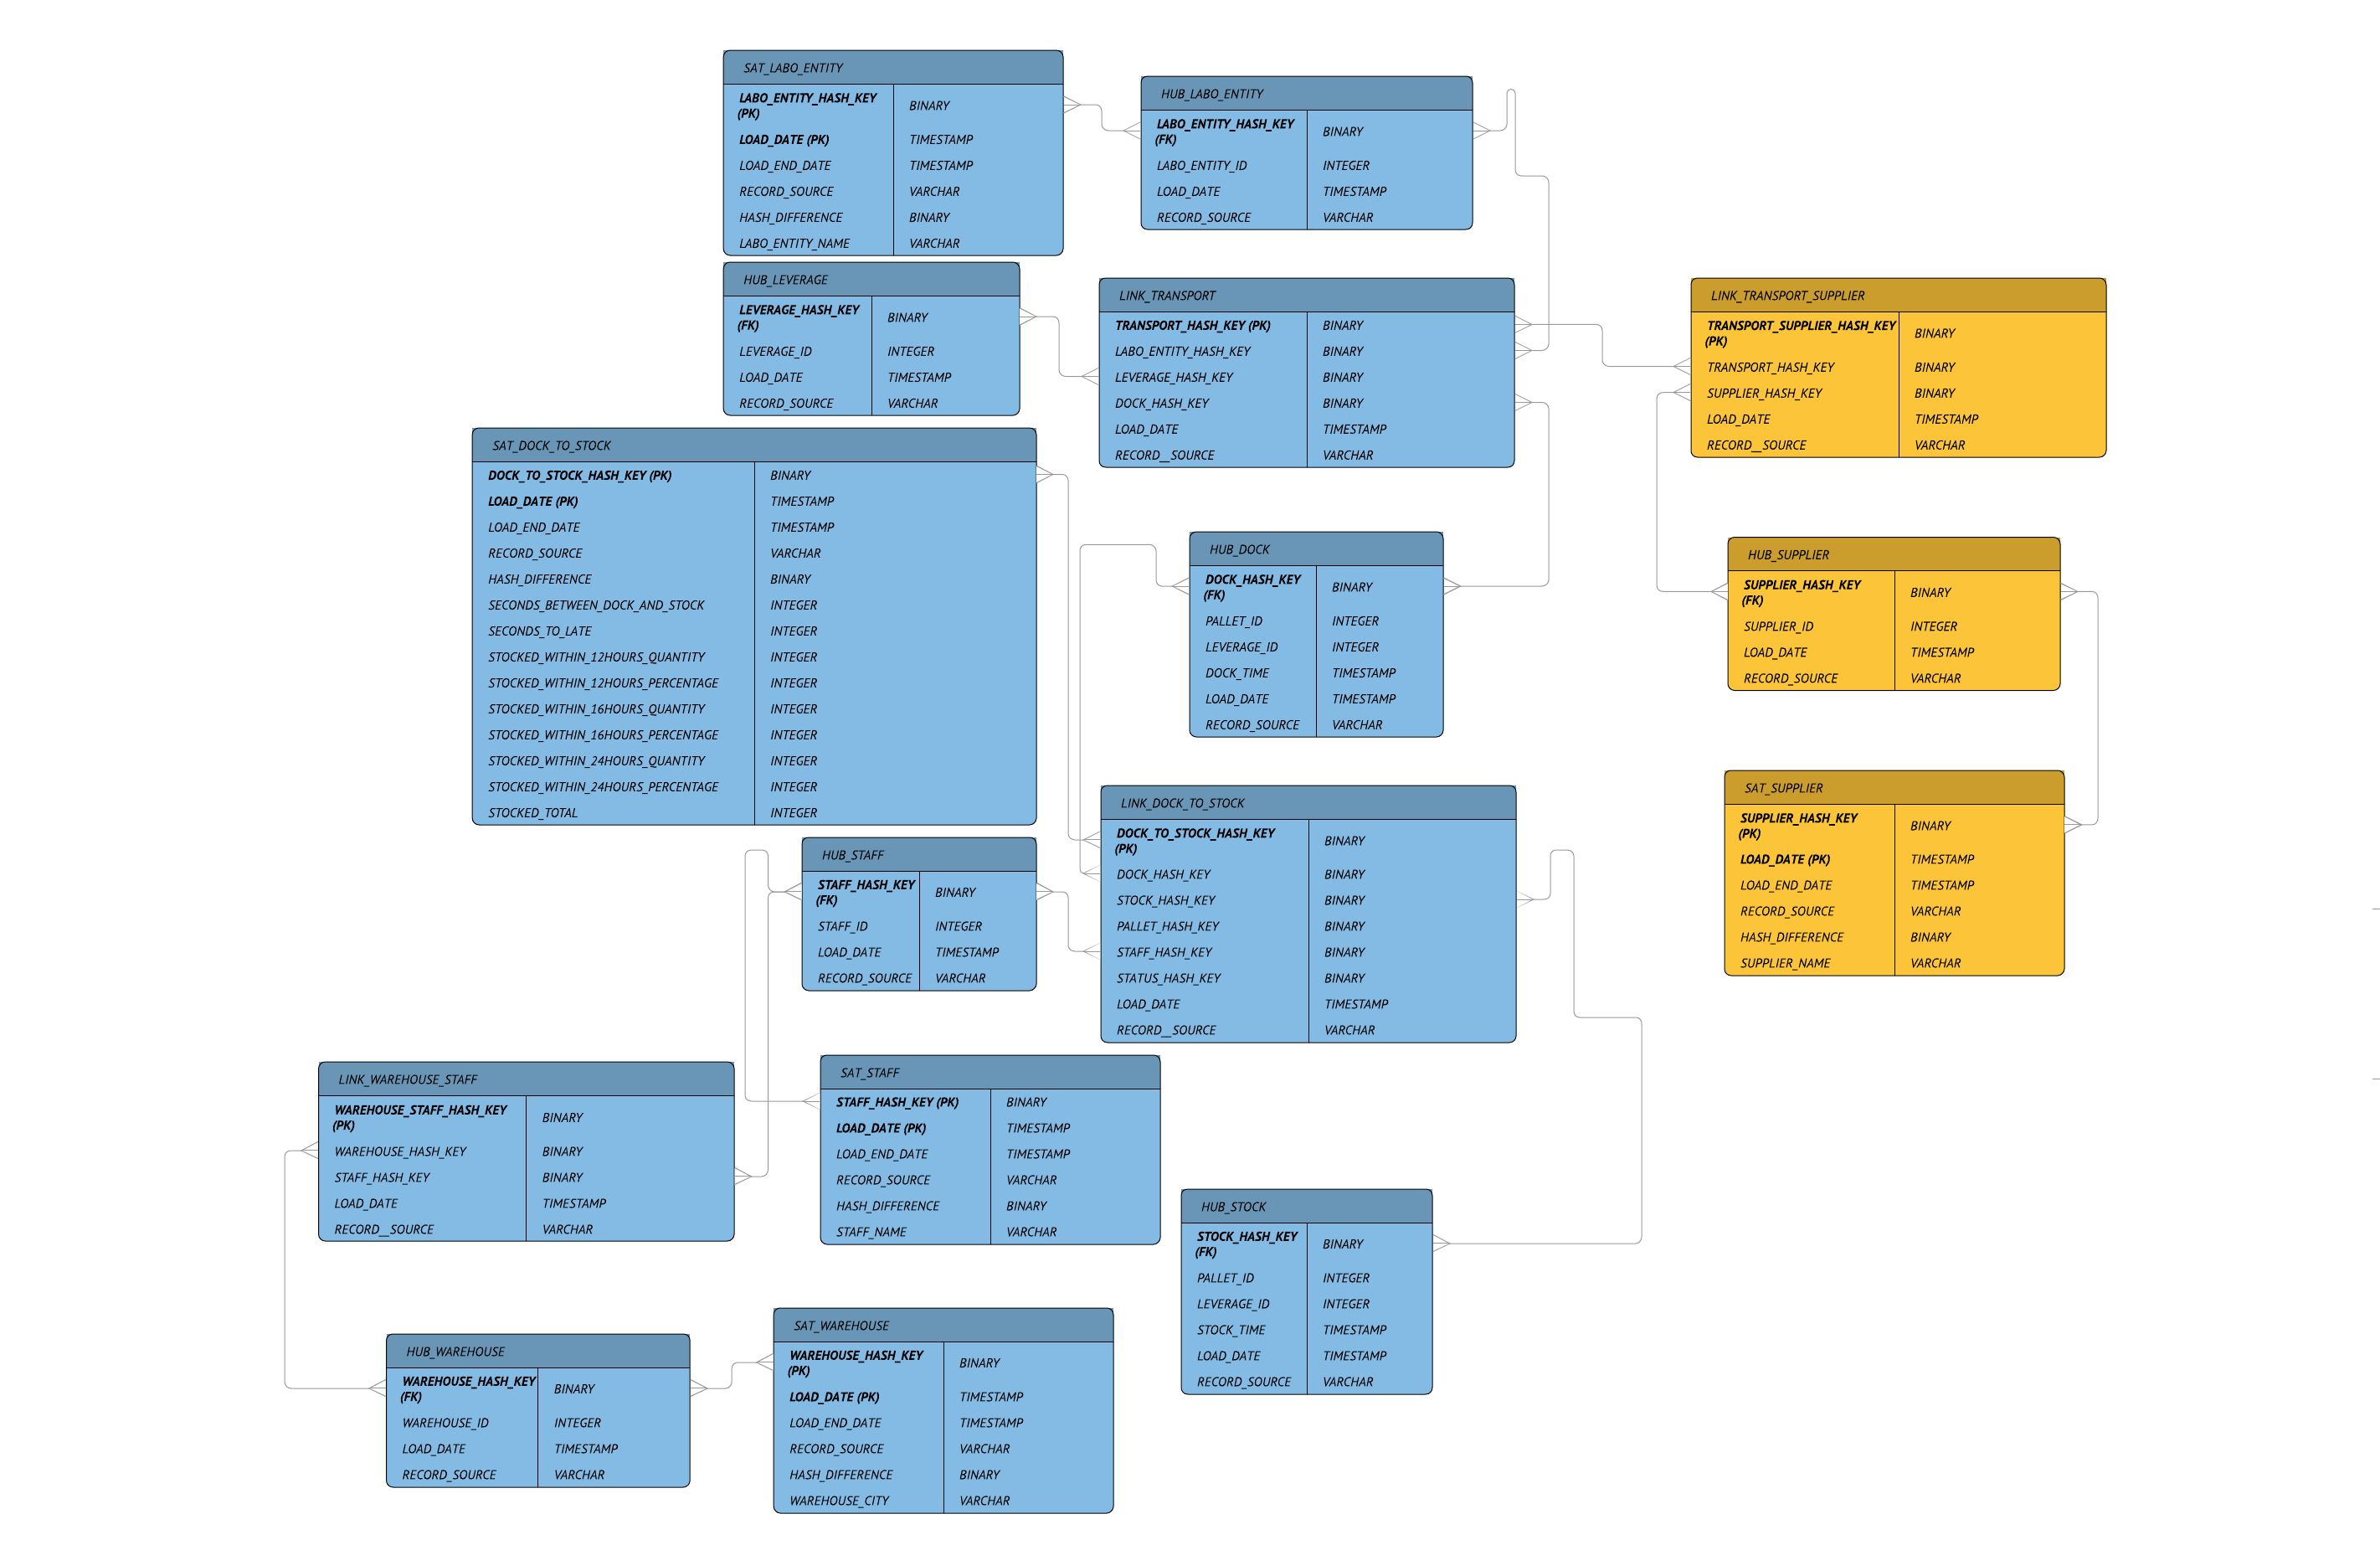
\includegraphics[scale=0.35]{../images/changedv.png}
	\caption{Het toevoegen van een nieuwe entiteit bij Data Vault (gemaakt via Lucidchart.com).}
	\label{fig:changedv}
\end{figure}

In figuur \ref{fig:changedv} wordt een nieuwe business requirement toegevoegd bij een bestaand Data Vault model. Hierbij wordt het bestaand model niet aangepast, maar er wordt wel een uitbreiding uitgevoerd. Er wordt een nieuwe link, hub \& sattelite toegevoegd (in het geel).

Deze manier van werken brengt een heel groot voordeel met zich mee op vlak van project management: via deze manier kan er gewerkt worden via de agile-manier, aangezien een toevoeging geen impact mag hebben op het bestaand data model.

Nieuwe business requirements toevoegen in het dimensioneel model is niet zo vanzelfsprekend. Een dimension ontwerpen en implementeren is eenvoudig, maar die nieuwe dimension zal moeten in relatie gezet worden met de centrale fact tabel. Dit betekent dat er een nieuwe key zal moeten toegevoegd worden in de fact tabel, en dat de huidige composite key dus zal moeten aangepast worden. De nieuwe toegevoegde key zal geen lege waarde mogen zijn.

\begin{figure}[h]
	\centering
	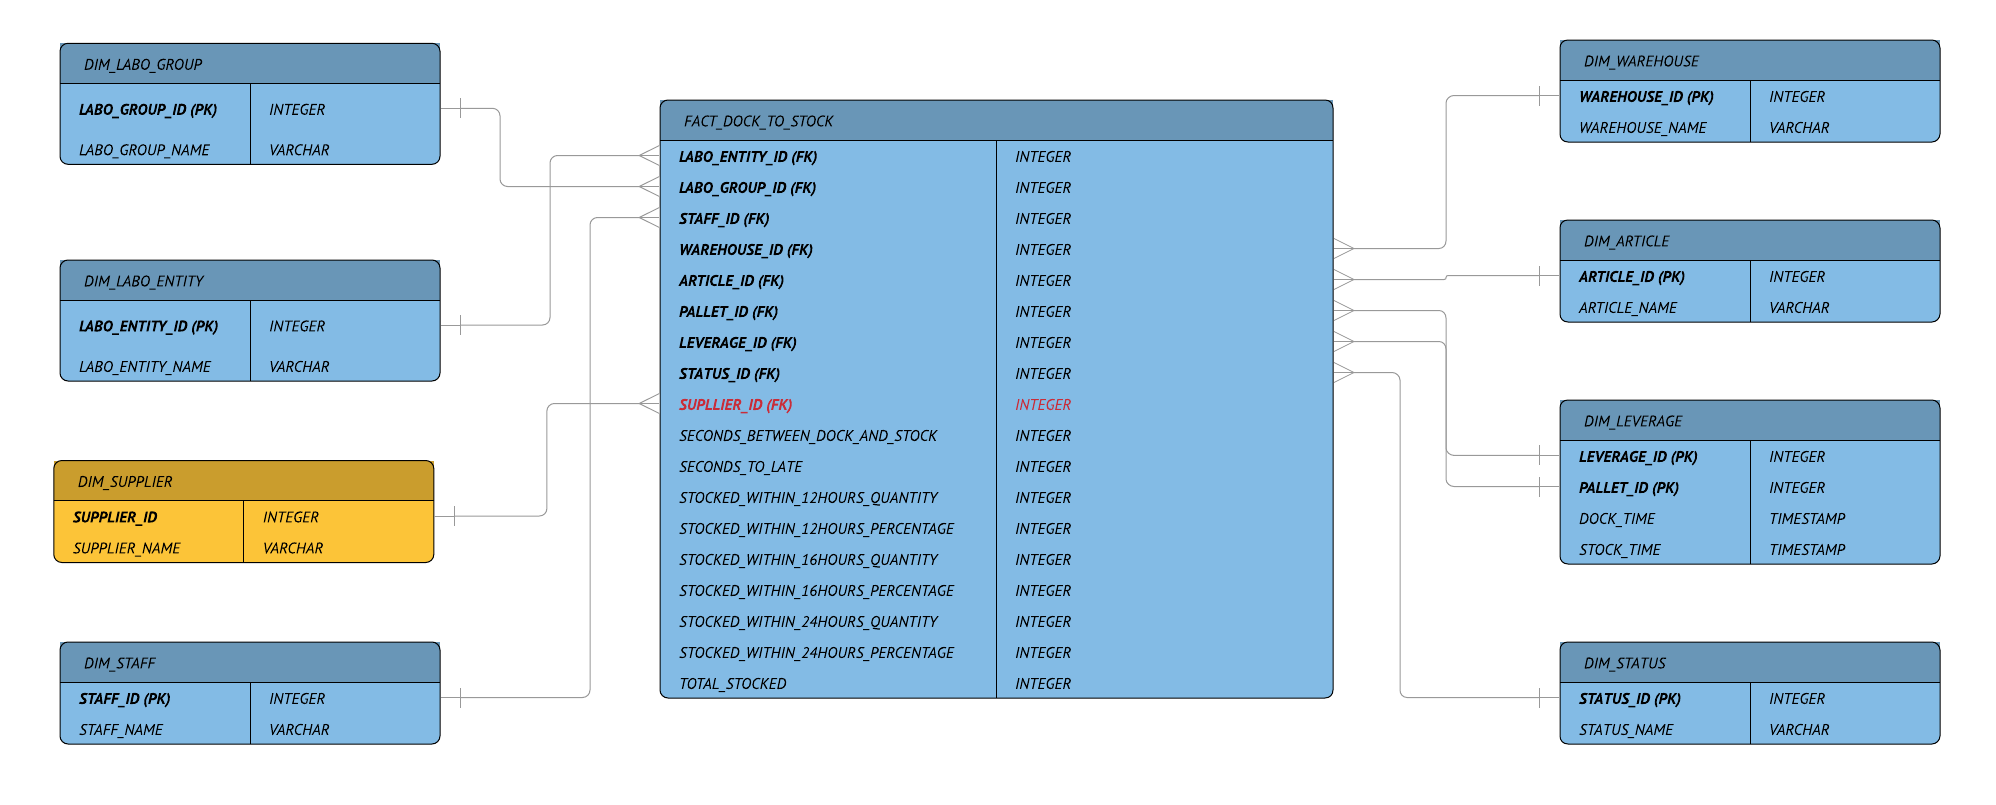
\includegraphics[scale=0.45]{../images/changedm.png}
	\caption{Het toevoegen van een nieuwe dimension bij een dimensioneel model (gemaakt via Lucidchart.com).}
	\label{fig:changedm}
\end{figure}

In figuur \ref{fig:changedm} wordt een nieuwe dimension (in het geel) toegevoegd aan het dimensioneel model. Het toevoegen van de nieuwe dimension heeft geen effect op de bestaande dimensions, maar wel in de fact tabel. In de fact tabel zal er een kolom moeten toegevoegd worden die de overeenkomstige keys bevat met de huidige data. Dit betekent dat het toevoegen van een nieuwe dimension wel degelijk een invloed heeft op het bestaande model en dat hier moeilijk via de agile methodologie kan gewerkt worden.

De structuur van een dimensioneel model ligt vast. Er is altijd een fact tabel die alle dimensions met elkaar verbindt. Het biedt geen opportuniteit om het schema te ontwerpen op basis van een business proces. Bij Data Vault is dit echter wel mogelijk. De flexibiliteit in de opbouw van een Data Vault is enorm hoog. Zo kan het model ontworpen worden op basis van een proces.

In een Data Vault model worden alleen maar many-to-many relaties gelegd door gebruik te maken van links. Dit is niet het geval bij het dimensioneel model. Door te werken met many-to-many relaties, verhoogt dit de flexibiliteit. Het nadeel door met many-to-many relaties te werken is dat het opvragen data langzamer zal verlopen.

Gegevens inladen in een data warehouse ontworpen aan de hand van een dimensioneel model verloopt deels serieel. Vooraleer de fact tabel ingeladen kan worden, moeten alle dimensions aanwezig zijn. Dit is niet zo bij een Data Vault model, hierin kan alles parallel ingeladen worden (omdat het gebruikt maakt van de business keys die de basis vormen van de hash key).

Het toevoegen van nieuwe bron gebeurt doorgaans ook eenvoudig bij Data Vault. Hiervoor moeten enkel nieuwe sattelites aangemaakt worden voor de benodigde data. Deze sattelites worden dan verbonden met de bijhoorende hubs. Opnieuw wordt het bestaande model niet aangepast. Bij het dimensioneel model moet hiervoor gebruik gemaakt worden van slow changing dimensions. Als dit principe niet van in het begin opgenomen is in het model, dan zal er heel wat moeite moeten gestopt worden in het toevoegen van een nieuwe databron (extra kolommen aanmaken, bestaande ETL aanpassen, ...).

De conclusie bij de vergelijking van Data Vault en het dimensioneel op basis van flexibiliteit is zeer duidelijk. De grote winnaar bij flexibiliteit is Data Vault, dat op alle vlakken van dit aspect duidelijk de betere keuze is.

\section{Schaalbaarheid}
Data warehouses bevatten doorgaans enorme hoeveelheden data. Bij de vergelijking tussen Data Vault en het dimensioneel model is het belangrijk om de schaalbaarheid van beide modellen te bestuderen. 

Het inladen van data in data warehouses kan bij enorme hoeveelheden data enorm veel tijd in beslag nemen. Bij sommige organisaties kan dit tot langer dan 12 uur duren. Daarom het een enorm voordeel indien er kan gebruik gemaakt worden van parallel inladen, wat het geval is bij Data Vault en niet bij het dimensioneel modelleren.

Op termijn zullen de volumes data bij een Data Vault groter zijn, aangezien dit model standaard extra informatie opneemt over de afkomst en tijdstip van extractie uit de bron. Bij Data Vault zal er meer opslagcapaciteiten nodig zijn in vergelijking met het dimensioneel model.

De conclusie bij de vergelijking rond schaalbaarheid is dat het Data Vault model enorm goed schaalt, maar als nadeel heeft dat er grotere opslagcapaciteiten nodig zijn.

\section{Audit}
Het bijhouden van historisatie en extra informatie over gegevens is voor sommige organisaties van groot belang. Denk maar bijvoorbeeld aan de bankensector, indien er iets fout is gelopen met een bepaalde transactie of indien men wilt te weten komen van waar bepaalde data opgehaald wordt, moet er hiervoor extra informatie aangeleverd kunnen worden. Historisatie wordt voornamelijk gebruikt bij gevoelige data. Andere voorbeelden van sectoren zijn: medische sector, overheden, verzekeringen, ....

In de Data Vault methodologie zit historisatie verwerkt. Er wordt extra informatie bijgehouden over waar de data exact vandaan komt (RECORD\_SOURCE), en wanneer de extractie van die data uit de bron gebeurd is (LOAD\_DATE). De reden waarom het tijdstip van extractie wordt bijgehouden en niet het tijdstip van het inladen van de gegevens in de data warehouse is omdat het ETL proces zeer lang kan duren en in de tussentijd de data in het bronsysteem al gewijzigd kan zijn. Via de Data Vault methodologie worden er in principe geen rijen gewijzigd (enkel de kolom LOAD\_END\_DATE), en worden nieuwere versies van data gewoon toegevoegd in de databank.

Bij het dimensioneel model wordt standaard noch de historisatie van data, noch extra informatie over de aangeleverde data niet bijgehouden. Voor historisatie bij het dimensioneel model kan gebruik gemaakt worden van slow changing dimensions. Indien gewenst kan er natuurlijk ook altijd geopteerd worden om deze extra informatie op te nemen door enkele kolommen toe te voegen. 

Er kan geconcludeerd worden dat Data Vault standaard historisatie toepast in hun model en dat er extra informatie (audit data) opgeslaan wordt over de data. Bij het dimensioneel model worden historisatie en het bijhouden van audit data niet opgenomen, maar het kan wel geïmplementeerd worden indien gewenst.
\section{Overzicht}
\begin{center}
	\renewcommand{\arraystretch}{2}%
	\begin{longtable}{  l  p{5,5cm}  p{5,5cm} }
		\ & \textbf{Data Vault} & \textbf{Dimensioneel model} \\ \hline
		Performantie & Data inladen gebeurt efficiënter, data opvragen gebeurt langzamer door de vele joins in het model. & Data lezen gebeurt vlot door een beperkt aantal joins, data inladen gebeurt langzamer door de afhankelijkheid van de fact tabel ten opzichte van de dimensions. \\ \hline
		Complexiteit & Hoge complexiteit, kennis nodig rond Data Vault. & Lage complexiteit, overzichtelijk. \\ \hline
		Flexibiliteit & Zeer hoge flexibiliteit, mogelijk om via de agile methode te werken. & Zeer lage flexibiliteit, vaste structuur. \\ \hline
		Schaalbaarheid & Goede schaalbaarheid door parallel inladen van de data. & Data inladen kan aanzienlijk langer duren doordat de fact tabel afhankelijk is van de dimensions en er niet parallel kan ingeladen worden.  \\ \hline
		Audit & Extra informatie aanwezig en de historiek van de data wordt bijgehouden. & Extra informatie niet aanwezig, indien gewenst kan dit wel toegevoegd worden. \\
		\caption{Overzicht van het vergelijkend onderzoek.}
		\label{tab:overzicht}
	\end{longtable}
\end{center}